\documentclass[a4paper,12pt]{article} % добавить leqno в [] для нумерации слева
\usepackage[a4paper,top=1.3cm,bottom=2cm,left=1.5cm,right=1.5cm,marginparwidth=0.75cm]{geometry}
%%% Работа с русским языком
\usepackage{cmap}					% поиск в PDF
\usepackage{mathtext} 				% русские буквы в фомулах
\usepackage[T2A]{fontenc}			% кодировка
\usepackage[utf8]{inputenc}			% кодировка исходного текста
\usepackage[english,russian]{babel}	% локализация и переносы
\usepackage{multirow}

\usepackage{graphicx}

\usepackage{wrapfig}
\usepackage{tabularx}

\usepackage{hyperref}
\usepackage[rgb]{xcolor}
\hypersetup{
colorlinks=true,urlcolor=blue
}

%%% Дополнительная работа с математикой
\usepackage{amsmath,amsfonts,amssymb,amsthm,mathtools} % AMS
\usepackage{icomma} % "Умная" запятая: $0,2$ --- число, $0, 2$ --- перечисление

%% Номера формул
\mathtoolsset{showonlyrefs=true} % Показывать номера только у тех формул, на которые есть \eqref{} в тексте.

%% Шрифты
\usepackage{euscript}	 % Шрифт Евклид
\usepackage{mathrsfs} % Красивый матшрифт

%% Свои команды
\DeclareMathOperator{\sgn}{\mathop{sgn}}

%% Перенос знаков в формулах (по Львовскому)
\newcommand*{\hm}[1]{#1\nobreak\discretionary{}
{\hbox{$\mathsurround=0pt #1$}}{}}

%% Графики
\usepackage{tikz}
\usepackage{pgfplots}
\pgfplotsset{compat=1.9}

\date{\today}

\begin{document}

\begin{titlepage}
	\begin{center}
		{\large МОСКОВСКИЙ ФИЗИКО-ТЕХНИЧЕСКИЙ ИНСТИТУТ (НАЦИОНАЛЬНЫЙ ИССЛЕДОВАТЕЛЬСКИЙ УНИВЕРСИТЕТ)}
	\end{center}
	\begin{center}
		{\large Физтех-школа аэрокосмических технологий}
	\end{center}
	
	
	\vspace{4.5cm}
	{\huge
		\begin{center}
			{\bf Отчёт о выполнении лабораторной работы 1.4.5}\\
			Изучение колебаний струны
		\end{center}
	}
	\vspace{1cm}
	\begin{center}
		{\large Соболевский Фёдор Александрович \\
			\vspace{0.2cm}
			Б03-109}
	\end{center}
	\vspace{8cm}
	\begin{center}
		Октябрь 2021
	\end{center}
\end{titlepage}

\section{Аннотация}

В работе изучены поперечные стоячие волны на тонкой натянутой струне.
Измерены собственные частоты колебаний струны, проверено условие образования
стоячих волн. Также измерена скорость распространения поперечных волн на струне и исследована её зависимость от натяжения струны. По результатам измерений вычислена погонная плотность струны. 

\section{Теоретические сведения}

Струной в акустике называют однородную тонкую гибкую упругую
нить. В данной работе
изучаются поперечные колебания стальной гитарной струны, натянутой горизонтально и закрепленной между двумя неподвижными зажимами.
Основное свойство струны — гибкость — обусловлено тем, что её поперечные размеры малы по сравнению с длиной. Это означает, что напряжение в струне может быть направлено только вдоль неё, и позволяет не
учитывать изгибные напряжения, которые могли бы возникать при поперечных деформациях (изгибе струны).

В натянутой струне возникает поперечная упругость, т.е. способность
сопротивляться всякому изменению формы, происходящему без изменения
объема. При вертикальном смещении произвольного элемента струны, возникают силы, действующие на соседние элементы, и в результате вся
струна приходит в движение в вертикальной плоскости. Передача возбуждения представляет собой поперечные
бегущие волны, распространяющиеся с некоторой скоростью в обе стороны от места возбуждения.

Рассмотрим гибкую однородную струну, в которой создано натяжение T, и получим дифференциальное уравнение, описывающее её малые
поперечные свободные колебания. Направим ось $ x $ вдоль струны в положении равновесия. Форму струны
будем описывать функцией $ y(x, t) $. Угол $ \alpha $ наклона касательной к
струне в точке относительно горизонтального направления в любой момент совпадает с углом наклона касательной к графику функции, то есть tg $ \alpha = \frac{\delta y}{\delta x} $

\begin{figure}[h]
\begin{center}
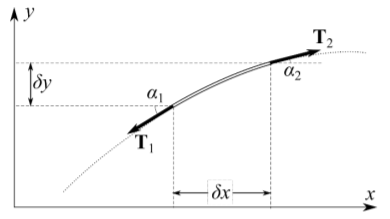
\includegraphics[width=0.6\textwidth]{1.4.5 waveEquation.PNG}
\end{center}
\caption{Схема колебаний струны на промежутке малой длины}
\label{fig:waveEquation}
\end{figure}

Рассмотрим элементарный участок струны, находящийся в точке $ x $,
имеющий длину $ \delta x $ и массу $ \delta m = \rho_l \delta x$ (см. рисунок \ref{fig:waveEquation}), где $ \rho_l $ [кг/м] — погонная плотность струны. При отклонении от равновесия
на выделенный элемент действуют силы натяжения $ T_1 $ и $ T_2 $, направленные
по касательной к струне. Их вертикальная составляющая будет стремиться
вернуть рассматриваемый участок струны к положению равновесия, придавая элементу некоторое вертикальное ускорение $ \frac{\delta^2 x}{\delta y^2}$. Угол $ \alpha $
зависит от координаты вдоль струны и различен в точках приложения
сил $ T_1 $ и $ T_2 $. Таким образом, второй закон Ньютона для вертикального движения элемента струны запишется в следующем виде:

\begin{equation}
    \delta m \frac{\delta^2 y}{\delta x^2} = -T_1 \sin{\alpha_1} + T_2 \sin{\alpha_2}
    \label{NewtonLaw}
\end{equation}

Учитывая, что рассматриваемые отклонения струны от положения
равновесия малы, можем сделать ряд упрощений:
\begin{enumerate}
    \item Длина участка струны в смещенном состоянии практически равна
длине участка в положении равновесия, поэтому добавочным
напряжением вследствие удлинения струны при деформации можно пренебречь. Следовательно, силы $ T_1 $ и $ T_2 $ по модулю равны силе
натяжения струны: $ T_1 \approx T_2 \approx T $ .
\item Углы наклона $ \alpha $ малы, поэтому tg $ \alpha \approx \sin \alpha \approx \alpha $, и, следовательно,
можно положить $ \alpha \approx \frac{\delta y}{\delta x}$.
\end{enumerate}

Разделим обе части уравнения движения \eqref{NewtonLaw} на  устремим размер элемента к нулю, $ \delta x $ → 0. Тогда уравнение \eqref{NewtonLaw} примет вид

\begin{equation}
    \rho_l \frac{\delta^2 y}{\delta t^2} = \frac{T_2 \sin{\alpha_2} - T_1 \sin{\alpha_1}}{\delta x} \approx T \frac{\alpha_2 - \alpha_1}{\delta x} \longrightarrow T \frac{\delta \alpha}{\delta x}
\end{equation}

Подставляя $ \alpha = \frac{\delta y}{\delta x}$ и величину с размерностью скорости

\begin{equation}
    u = \sqrt{\frac{T}{\rho_l}},
    \label{sped}
\end{equation}

получаем уравнение свободных малых поперечных колебаний
струны, или волновое уравнение:

\begin{equation}
    \frac{\delta^2 y}{\delta x^2} = u^2 \frac{\delta^2 y}{\delta t^2}
    \label{waveEquation}
\end{equation}

Покажем, что введённая величина $ u $ - скорость распространения волны на струне. Рассмотрим произвольную функцию вида $ f(x - ut) $, описывающую возмущение струны произвольной формы, движущееся по струне поступательно со скоростью $ u $ вдоль оси $ x $, не меняя своей формы. При подстановке её в уравнение \eqref{waveEquation} получается верное равенство:

\begin{equation}
    \frac{\delta^2 f}{\delta x^2} = (-u)^2 f'' = u^2 \frac{\delta^2 f}{\delta t^2},
\end{equation}

где $ f'' $ - производная функции по аргументу $ (x - ut) $.

Общее решение уравнения \eqref{waveEquation} представимо в виде суммы двух волн произвольной формы, бегущих в противоположные стороны со скоростями $ \pm u $:

\begin{equation}
    y(x, t) = y_1(x - ut) + y_2(x + ut),
\end{equation}

где $ y_1 $ и $ y_2 $ - произвольные функции, вид которых
в конкретной задаче определяется из начальных и граничных условий. В случае гармонических волн решение представляется в виде

\begin{equation}
    y(x, t) = a\cos{(\omega t - kx)} + b\cos{(\omega t + kx)}.
    \label{harmonicSolution}
\end{equation}

Выражение \eqref{harmonicSolution} представляет собой линейную комбинацию (суперпозицию)
двух гармонических волн с амплитудами $ a $ и $ b $, бегущих навстречу друг
другу со скоростью

\begin{equation}
    u = \frac{\omega}{k} = \lambda \nu ,
\end{equation}

где $ \lambda $ - длина волны, $ \nu $ - частота, $ k $ - волновое число (пространственная частота). При возбуждении струны периодической гармонической силой её колебания будут описываться формулой \eqref{harmonicSolution}.

Найдем вид свободных колебаний струны с закрепленными концами.
Пусть струна закреплена в точках $ x = 0 $ и $ x = l $. Концы струны не колеблются, поэтому $ y(0, t) = 0 $ и $ y(L, t) = 0$ при любых $ t $. Используя формулу \eqref{harmonicSolution}, находим

\begin{equation}
    y(0, t) = a\cos{\omega t} + b\cos{\omega t} = 0,
\end{equation}

откуда следует, что $ a = -b $. После тригонометрических преобразований выражение \eqref{harmonicSolution} примет вид

\begin{equation}
    y(x, t) = 2a\sin{kx} \cdot \sin{\omega t}
    \label{staticWaves}
\end{equation}

Колебания струны, описываемые данной функцией, называются стоячими волнами. Из выражения \eqref{staticWaves} видно, что стоячая волна может быть получена как суперпозиция двух гармонических бегущих навстречу друг другу волн с равными амплитудами. 

Точки струны, в которых $ \sin{kx} = 0 $, в любой момент времени неподвижны. Такие точки называются узлами стоячей волны. Остальные участки струны совершают в вертикальной плоскости гармонические колебания с частотой $ \nu = \frac{\omega}{2\pi} = \frac{u}{\lambda} $. Амплитуда колебаний распределена вдоль струны по гармоническому закону: $ y_0(x) = 2a\sin{kx}$. В точках,
где $ \sin{kx} = 1 $, амплитуда колебаний максимальна, такие точки называются пучностями.

Используя второе граничное условие $ y(L, t) = 0 $, найдём условие образования на струне стоячих волн: $ y(x, t) = 2a\sin{kL} \cdot \sin{\omega t}$, откуда

\begin{equation}
    \sin{kL} = 0  \longrightarrow kL = \frac{\pi n}{2}, n \in \mathbb{N}
\end{equation}

Таким образом, стоячие волны на струне с закреплёнными концами образуются, только если на длине струны укладывается целое число полуволн:

\begin{equation}
    \lambda_n = \frac{2L}{n}.
    \label{staticWaveReq}
\end{equation}

\begin{figure}
    \centering
    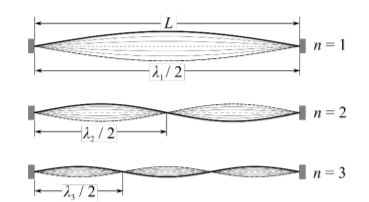
\includegraphics[width = 0.6\textwidth]{1.4.5 staticWaves.PNG}
    \caption{Стоячие волны для $ n = 1, 2, 3 $}
    \label{fig:staticWaves}
\end{figure}

На рисунке \ref{fig:staticWaves} показана картина стоячих волн для $ n = 1, 2, 3 $. Число $ n $ показывает число пучностей колеблющейся струны (при этом число узлов - $ n + 1 $. Поскольку длина волны однозначно связана с её частотой, струна может
колебаться только с определёнными частотами:

\begin{equation}
    \nu_n = \frac{u}{\lambda_n} = \frac{n}{2L}\sqrt{\frac{T}{\rho_l}}
    \label{ownFrequency}
\end{equation}

Разрешённые частоты $ \nu_n $ называют собственными частотами колебаний струны. Таким образом, спектр собственных частот тонкой струны определён её погонной плотностью $ \rho_l $, внешней силой натяжения $ T $ и длиной
струны L и не зависит от модуля Юнга материала струны. 

\begin{figure}
    \centering
    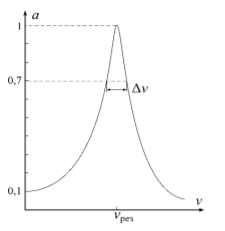
\includegraphics[width = 0.3\textwidth]{1.4.5 AFC.PNG}
    \caption{АЧХ вынужденных колебаний}
    \label{fig:AFC}
\end{figure}

При колебаниях реальной струны всегда имеет место потеря энергии
(часть теряется вследствие трения о воздух; другая часть уходит через неидеально закрепленные концы струны и т.д.). Поддержание незатухающих
колебаний в струне может осуществляться точечным источником, в качестве которого в данной работе используется электромагнитный вибратор.
Для эффективной раскачки колебаний используется явление резонанса
— вынуждающая частота $ \nu $ должна совпадать с одной из собственных частот струны $ \nu_n $. Когда потери энергии в точности компенсируются энергией, поступающей от вибратора, колебания струны становятся стационарными и на ней можно наблюдать стоячие волны. 
Оценить затухание колебаний можно через добротность колебательной системы. В случае вынужденных колебаний расчёт добротности производится по амплитудно-частотной характеристике (АЧХ) колебаний (см. рисунок \ref{fig:AFC}). Для расчётов в данном опыте воспользуемся известным из теории колебаний результатом: добротность колебательной системы связана с резонансной частотой $ \nu_\text{рез} $ и шириной резонансной кривой $ \Delta \nu $ соотношением 

\begin{equation}
    Q = \frac{\nu_\text{рез}}{\Delta \nu}
\end{equation}

где ширина резонансной кривой $ \Delta \nu $ измеряется на уровне амплитуды, составляющей 0,7 от амплитуды в резонансе.

\begin{figure}
    \centering
    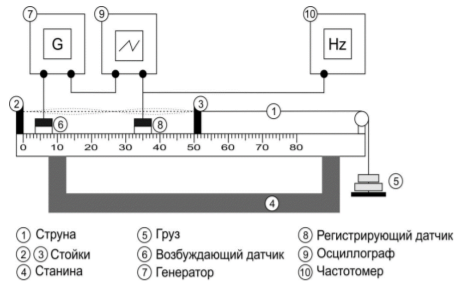
\includegraphics[width = 0.6\textwidth]{1.4.5 setup.PNG}
    \caption{Схема экспериментальной установки}
    \label{fig:setup}
\end{figure}

Схема экспериментальной установки приведена на рисунке \ref{fig:setup}. Стальная гитарная струна \textbf{1} закрепляется в горизонтальном положении между двумя стойками с зажимами \textbf{2} и \textbf{3}, расположенными на массивной станине \textbf{4}. Один конец струны
закреплен в зажиме \textbf{2} неподвижно. К противоположному концу струны, перекинутому через блок, прикреплена платформа с грузами \textbf{5}, создающими
натяжение струны. Зажим \textbf{3} можно передвигать по станине, устанавливая
требуемую длину струны. Возбуждение и регистрация колебаний струны
осуществляются с помощью электромагнитных датчиков (вибраторов),
расположенных на станине под струной. Электромагнитный датчик \textbf{6} подключен к звуковому генератору \textbf{7} и служит для возбуждения колебаний струны, частота которых измеряется с помощью частотомера \textbf{10} (в некоторых установках частотомер встроен в генератор). Колебания струны регистрируются с помощью электромагнитного датчика \textbf{8}, сигнал с которого
передается на вход осциллографа \textbf{9}. Разъёмы, через которые датчики с помощью кабелей соединяются с генератором и осциллографом, расположены на корпусе станины.

\section{Оборудование и инстументальные погрешности}
\textbf{Оборудование:} струна, закреплённая на станине с помощью подвижной и неподвижной стоек, набор грузов; подвес для грузов, подвешенный через неподвижный блок к струне; возбуждающий и регистрирующий электромагнитные датчики, звуковой генератор, осциллограф, частотометр. \\
Измерительные приборы, используемые в данной работе (осциллограф, частотометр), достаточно точные и имеют небольшие систематические погрешности по сравнению со случайной ошибкой измерений, поэтому ими в данной работе можно пренебречь.

\section{Результаты измерений и обработка экспериментальных данных}

\subsection{Предварительные расчёты}

Перед началом работы были проведены предварительные расчёты, чтобы оценить первую собственную частоту колебаний струны. Масса подвеса и грузов в первом опыте $ m_1 = 919,4 $ г, сила натяжения струны $ T_1 = m_1 g = 9,01 $ Н. Указанное на установке значение погонной плотности струны $ \rho_l = 568,4 $ мг/м. Из формулы \eqref{ownFrequency} первая собственная частота колебаний струны

\begin{equation}
    \nu_\text{пред} = \frac{1}{2L}\sqrt{\frac{T}{\rho_l}} \approx 125,9 \text{ Гц}.
\end{equation}

Экспериментальное значение $ \nu_1 = 124,4 $ Гц достаточно близко к вычисленному. Отсюда видно, что описанные теоретические закономерности в данном опыте применимы. 

\subsection{Измерение собственных частот струны}

Измерение собственных частот было проведено для 5 различных значений натяжения $ T $ и проводилось с помощью осциллографа. При нахождении подходящей частоты колебания струны были визуально самыми большими. Это говорит о достаточной для проведения эксперимента точности данного прибора.
Результаты измерений представлены в таблице \ref{tab:freaqs}.

\begin{table}[h]
    \centering
    \begin{tabular}{|c|c|c|c|c|c|c|c|}
    \hline
    № опыта & $ m $ подвеса с грузом, г & $ T $, Н & $ \nu_1 $, Гц & $ \nu_2 $, Гц & $ \nu_3 $, Гц & $ \nu_4 $, Гц & $ \nu_5 $, Гц \\ 
    \hline
    1 & 919,4 & 9,01 & 124,4 & 260,4 & 376,2 & 503,0 & 632,6 \\
    \hline
    2 & 1420,8 & 13,92 & 157,7 & 317,3 & 477,5 & 632,4 & 793,7 \\
    \hline
    3 & 1915,9 & 18,78 & 181,4 & 363,7 & 546,5 & 728,6 & 910,2 \\
    \hline
    4 & 2407,0 & 23,59 & 203,4 & 407,5 & 611,7 & 816,7 & 1020,7 \\
    \hline
    5 & 2863,2 & 28,06 & 220,9 & 443,4 & 668,1 & 889,4 & 1116,0 \\
    \hline
    \end{tabular}
    \caption{Собственные частоты струны для разных натяжений}
    \label{tab:freaqs}
\end{table}

\subsection{Вычисление скоростей распространения волн}

Для нахождения скоростей $ u $ распространения волн на струне был использован метод построения наилучших прямых. Зависимость $ \nu_n $ от $ n $ можно найти из выражений \eqref{sped} и \eqref{ownFrequency}:

\begin{equation}
    \nu_n = \frac{u}{2L} n
\end{equation}

Данная зависимость линейная. Пусть $ k = \frac{u}{2L} $. Построим прямые, проходящие через начало координат (см. рисунок \ref{graph}), и  найдём для каждого значения натяжения $ T $ коэффицент $ k $ методом наименьших квадратов: 

\begin{equation}
    k = \frac{\langle n\nu_n\rangle}{\langle n^2\rangle}
\end{equation}

Погрешность вычисления $ k $ найдём как

\begin{equation}
    \sigma_k = \sqrt{\frac{1}{N - 1}(\frac{\langle\nu_n^2\rangle}{\langle n^2\rangle} - k^2)}
\end{equation}

\begin{figure}
\centering
\resizebox {0.7\textwidth} {!} {
\begin{tikzpicture}
\begin{axis}[ xlabel = {$ n $}, ylabel = {$ \nu_n $, Гц}, xmin = 0, xmax = 6.5, ymin = 0, ymax = 1300 ]
\addplot[color=black, mark=square, only marks] coordinates{(1, 124.4)(2, 260.4)(3, 376.2)(4, 503)(5, 632.6)};

\addplot[color=black, mark=x, only marks] coordinates{(1, 157.7)(2, 317.3)(3, 477.5)(4, 632.4)(5, 793.7)};

\addplot[color=black, mark=o, only marks] coordinates{(1, 181.4)(2, 363.7)(3, 546.5)(4, 728.6)(5, 910.2)};

\addplot[color=black, mark=star, only marks] coordinates{(1, 203.4)(2, 407.5)(3, 611.7)(4, 816.7)(5, 1020.7)};

\addplot[color=black, mark=triangle, only marks] coordinates{(1, 220.9)(2, 443.4)(3, 668.1)(4, 889.4)(5, 1116)};
\legend{$ T_1 $, $ T_2 $, $ T_3 $, $ T_4 $, $ T_5 $}
\addplot[color=blue] {126.3*x};
\addplot[color=red] {158.6*x};
\addplot[color=blue] {182.07*x};
\addplot[color=red] {204.06*x};
\addplot[color=blue] {222.72*x};
\end{axis}
\end{tikzpicture}
}
\caption{Зависимость $ \nu_n $ от $ n $}
\label{graph}
\end{figure}

Найденные значения $ k $, $ u $ и их погрешности при разных $ T $ представлены в таблице \ref{tab:velocys}.

\begin{table}[h]
    \centering
    \begin{tabular}{|c|c|c|c|c|c|}
    \hline
    № опыта & $ T $, Н & $ k $, Гц & $ \sigma_k $, Гц & $ u $, м/с & $ \sigma_u $, м/с \\ 
    \hline
    1 & 9,01 & 126,3 & 0,6 & 126,3 & 0,6 \\
    \hline
    2 & 13,92 & 158,60 & 0,19 & 158,60 & 0,19 \\
    \hline
    3 & 18,78 & 182,07 & 0.06 & 182.07 & 0.06 \\
    \hline
    4 & 23,59 & 204,06 & 0.08 & 204.06 & 0.08 \\
    \hline
    5 & 28,06 & 222,72 & 0,26 & 222,72 & 0,26 \\
    \hline
    \end{tabular}
    \caption{Скорость распространения волн на струне при разных натяжениях}
    \label{tab:velocys}
\end{table}

\subsection{Вычисление погонной плотности}

По найденным значениям скоростей $ u $ можно вычислить погонную плотность стали, снова применяя метод построения наилучших прямых. Зависимость $ u^2 $ от $ T $ можно найти из выражения \eqref{sped}:

\begin{equation}
    u^2 = \frac{1}{\rho_l} T.
\end{equation}

\begin{figure}
\centering
\resizebox {0.7\textwidth} {!} {
\begin{tikzpicture}
\begin{axis}[ xlabel = {$ T $, Н}, ylabel = {$ u^2 $, $10^3\cdot \text{м}^2/\text{с}^2 $}, xmin = 0, xmax = 30, ymin = 0, ymax = 55 ]
\addplot[color=black, mark=x, only marks] coordinates{(9.01, 15.95169)(13.92, 25.15396)(18.78, 33.149485)(23.59, 41.64048)(28.06, 49.6042)};
\addplot[color=blue] coordinates{(0, 0)(30, 53.118)};
\end{axis}
\end{tikzpicture}
}
\caption{Зависимость $ u^2 $ от $ T $}
\label{graphtoo}
\end{figure}

Данная зависимость также линейная. Пусть $ k = \frac{1}{\rho_l} $. Построим прямую, проходящую через начало координат (см. рисунок \ref{graphtoo}), и  найдём для неё коэффицент $ k $ и $ \sigma_k $ методом наименьших квадратов: 
%%%%%%%%%%%%%%%%%%%%%%%%%%%%%%%%%%%%%%%%%%%%%%%%%%%%%%%%%%%%%%%%%%%%%%%%%%%%
\begin{equation}
    k = \frac{\langle T u^2 \rangle}{\langle T^2 \rangle} = 1770,6 \text{ м/кг},
\end{equation}

\begin{equation}
    \sigma_k = \sqrt{\frac{1}{N - 1}(\frac{\langle u^4 \rangle}{\langle T^2 \rangle} - k^2)} = 6,0 \text{ м/кг}.
\end{equation}

Отсюда значение $ \rho_l = \frac{1}{k} = 564,7 \cdot 10^{-6} \text{кг/м}$. Погрешность определения погонной плотности $ \sigma_\rho $ связана с $ \sigma_k $ соотношением 

\begin{equation}
    (\frac{\sigma_\rho}{\rho_l})^2 = (-1)^2 (\frac{\sigma_k}{k})^2, \sigma_\rho = \frac{\rho_l}{k} \sigma_k = 1,9 \cdot 10^{-6} \text{ кг/м}.
\end{equation}

Окончательный результат:

\begin{itemize}
    \item $ \rho_l = (564,7 \pm 1,9)\cdot 10^{-6} \text{ кг/м}$.
\end{itemize}

\subsection{Вычисление добротности системы}

В пятом опыте ($ T = 28,632 $ Н) первая резонансная частота составила $ \approx 222$ Гц. Ширина резонансной кривой для данного значения составила $ 0,28 $ Гц. Отсюда добротность струны как колебательной системы

\begin{equation}
    Q = \frac{\nu_\text{рез}}{\Delta \nu} \approx 792,86
\end{equation}

Данное значение достаточно высокое для колебательной системы, исследуемой в учебных целях, что говорит об отсутствии необходимости делать поправку на потери энергии в системе.

\section {Обсуждение результатов и вывод}

Полученный результат $ \rho_l = 564,7 \cdot 10^{-6} \text{ кг/м}$ отличается от указанного на установке (измеренного непосредственным взвешиванием, $ \rho_l = 568,4 \cdot 10^{-6} \text{ кг/м}$) меньше, чем на $ 2\sigma_\rho $. Относительная погрешность измерений ($ \epsilon_\rho = 0,65 \% $) также невелика. Это говорит о применимости данного метода при измерении погонной плотности наравне с прямым взвешиванием. Все рассмотренные теоретические закономерности выполнились в пределах точности эксперимента. 

\end{document}
